\chapter{Từ nguyên lý tương đương đến tensor}

Thuyết tương đối rộng thường được viết tắt là GR, mặc dù thuyết tương đối hẹp hiếm khi được gọi là SR. Chữ viết tắt kém quan trọng hơn quyết định bắt đầu từ ngay khởi đầu. Con đường trực tiếp nhất là con đường Einstein đã đi: bắt đầu từ một quan sát vật lý đủ đơn giản để có thể cảm nhận được trong một thang máy, khai thác nó cho đến khi các hệ quả của nó trở nên không thể tránh khỏi, và chỉ khi đó mới giới thiệu hình học.

Quan sát đầu tiên là nguyên lý tương đương. Hấp dẫn và gia tốc là không thể phân biệt được một cách cục bộ. Từ cục bộ rốt cuộc sẽ gánh gần như toàn bộ sức nặng của mệnh đề này. Tuy nhiên, trước khi bổ sung sự hạn định ấy, ta nên xem mệnh đề chưa hạn định đã có thể làm được gì.

\section{Thang máy như một phép biến đổi tọa độ}

Các giáo trình thường thay thang máy của Einstein bằng một con tàu tên lửa. Ở đây thang máy thích hợp hơn vì gia tốc của nó là điều quen thuộc. Gọi \(z\) đo độ cao trong một hệ gắn với mặt đất, và gọi \(z'\) đo độ cao tính từ sàn thang máy. Nếu sàn có độ cao \(L(t)\), thì cùng một sự kiện có tọa độ
\begin{equation}
 z'=z-L(t),\qquad t'=t,\qquad x'=x.
\label{eq:elevator-map}
\end{equation}
Tọa độ ngang không đổi vì thang máy không trượt sang bên. Việc lấy \(t'=t\) cố ý tạm thời gác thuyết tương đối hẹp sang một bên.

\begin{classroomqa}
\audiencequestion{Làm sao một khóa học về thuyết tương đối rộng lại có thể bắt đầu bằng cách bỏ qua thuyết tương đối hẹp?}
\lecturerresponse{Có một chế độ trong đó hấp dẫn là quan trọng trong khi mọi vận tốc vẫn nhỏ so với \(c\). Vì vậy, mối liên hệ hấp dẫn--gia tốc có thể được tách riêng trong cơ học Newton rồi sau đó kết hợp với hình học Minkowski. Đây là một lựa chọn về cách triển khai, không phải một khẳng định rằng lý thuyết cuối cùng là phi tương đối tính. \lecturetimestamp{00:05:33}}
\end{classroomqa}

Đối với hai hệ quán tính, thang máy chuyển động đều,
\begin{equation}
 L(t)=vt,\qquad z'=z-vt.
\label{eq:galilean-elevator}
\end{equation}
Các gốc tọa độ đã được chọn trùng nhau tại \(t=0\). Trên bảng, hình vẽ thang máy được đặt cạnh cả ba quan hệ tọa độ để các ký hiệu không bao giờ mất đi ý nghĩa vật lý của chúng.

\begin{figure}[H]
\centering
\includegraphics[width=\linewidth]{lecture_01_figure_01.png}
\caption{Tọa độ của thang máy sau khi chuyên biệt hóa thành trường hợp vận tốc đều \(L(t)=vt\).}
\par\smallskip
\textit{Khung hình bài giảng: 00:09:10.}
\end{figure}

Chỉ xét thành phần thẳng đứng của định luật Newton,
\begin{equation}
 F=m\ddot z.
\label{eq:newton-unprimed}
\end{equation}
Lực có thể đến từ một sợi dây, một điện trường, hoặc bất kỳ tương tác thông thường nào khác. Lấy đạo hàm hai lần của \eqref{eq:galilean-elevator} cho
\(\ddot z'=\ddot z\), và do đó
\begin{equation}
 F=m\ddot z'.
\label{eq:newton-primed-inertial}
\end{equation}
Dạng của định luật không đổi. Phép tính sơ đẳng này làm lộ rõ nội dung có hiệu lực của sự tương đương giữa các hệ quán tính: một phép biến đổi tọa độ tuyến tính biến chuyển động đều thành chuyển động đều.

\begin{figure}[H]
\centering
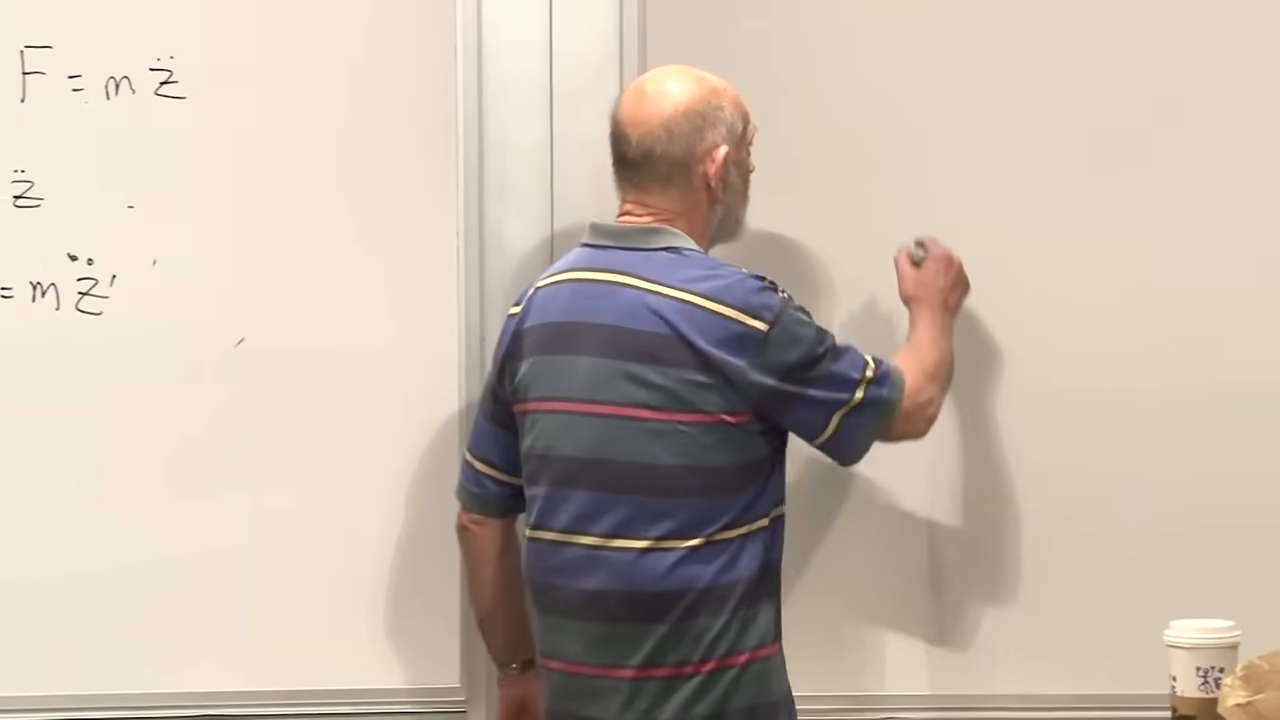
\includegraphics[width=\linewidth]{lecture_01_figure_02.png}
\caption{Phương trình Newton trong hai hệ tọa độ chuyển động đều.}
\par\smallskip
\textit{Khung hình bài giảng: 00:11:50.}
\end{figure}

Bây giờ cho thang máy gia tốc hướng lên trên với \(g\) không đổi:
\begin{equation}
 L(t)=\frac12gt^2,\qquad
 \dot L=gt,\qquad
 \ddot L=g.
\end{equation}
Phép biến đổi tọa độ trở thành
\begin{equation}
 z'=z-\frac12gt^2,
\qquad
 \ddot z'=\ddot z-g.
\label{eq:accelerated-map}
\end{equation}
Thế vào định luật Newton cho
\begin{equation}
 F=m(\ddot z'+g),
\qquad
 m\ddot z'=F-mg.
\label{eq:fictitious-gravity}
\end{equation}
Phép suy ra này bao gồm một phép kiểm tra dấu trực tiếp hữu ích: \(+mg\) trước hết xuất hiện ở vế gia tốc và chỉ trở thành \(-mg\) khi được chuyển sang vế lực. Hướng cuối cùng là hướng xuống trong hệ mà sàn của nó đang gia tốc đi lên.

\begin{figure}[H]
\centering
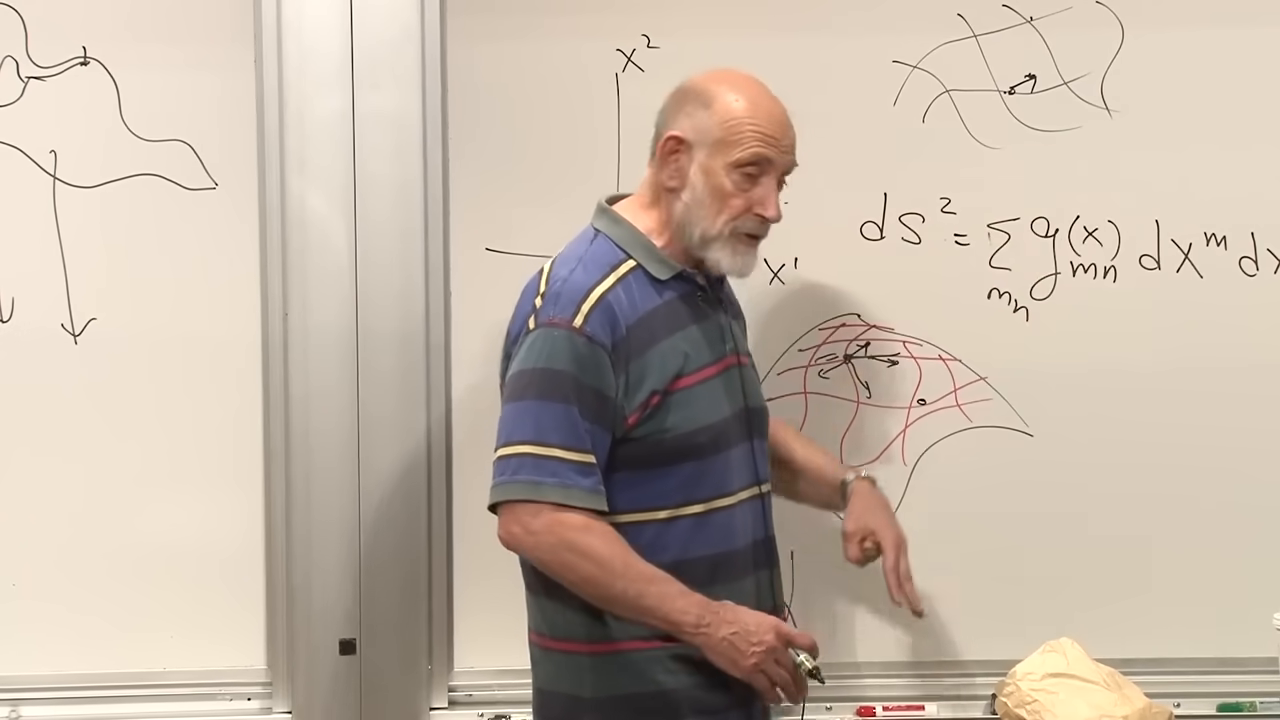
\includegraphics[width=\linewidth]{lecture_01_figure_03.png}
\caption{Phép biến đổi gia tốc và lực hư cấu thu được \(-mg\).}
\par\smallskip
\textit{Khung hình bài giảng: 00:15:35.}
\end{figure}

Hạng mới trông giống hấp dẫn vì một lý do chính xác: nó tỉ lệ với khối lượng. Vì đáp ứng quán tính cũng tỉ lệ với khối lượng, khối lượng triệt tiêu khỏi phương trình chuyển động. Một vật rơi tự do đi theo cùng một quỹ đạo bất kể khối lượng của nó. Chẳng hạn, trong gần đúng vật thử, quỹ đạo của Trái Đất được quyết định bởi vị trí và vận tốc của nó trong trường của Mặt Trời, chứ không phải bởi chính khối lượng của Trái Đất.

Trước Einstein, sự giống nhau này có thể bị gạt đi như một điều hiếu kỳ. Ngược lại, Einstein nâng nó lên thành một nguyên lý: không thí nghiệm cơ học cục bộ nào có thể phân biệt một trường hấp dẫn đồng nhất với một hệ quy chiếu gia tốc thích hợp.

\section{Đường thẳng, tọa độ cong, và ánh sáng}

Biểu diễn \(t\) theo phương thẳng đứng và \(z\) theo phương ngang. Với \(z'=z-vt\), các đường \(z'\) không đổi là những đường thẳng song song. Các đường thế giới thẳng vẫn thẳng vì phép biến đổi tọa độ là tuyến tính.

\begin{figure}[H]
\centering
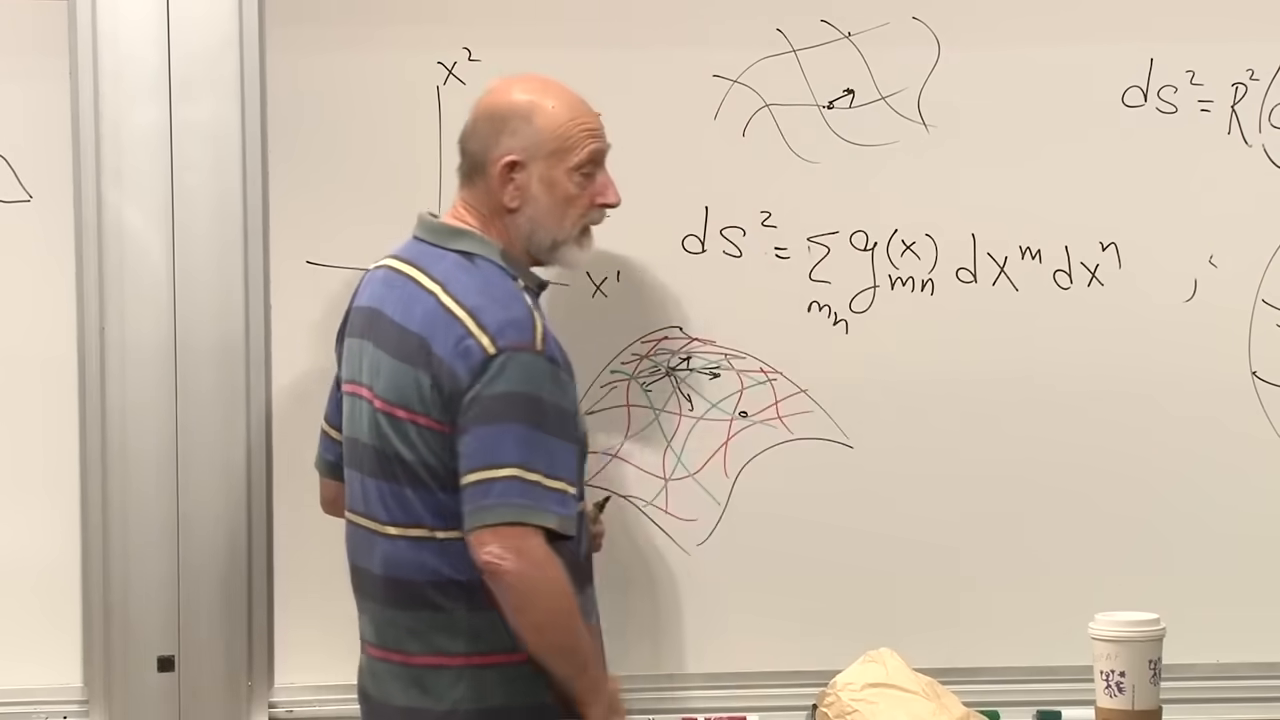
\includegraphics[width=\linewidth]{lecture_01_figure_04.png}
\caption{Một lưới không-thời gian tuyến tính cho các tọa độ chuyển động đều.}
\par\smallskip
\textit{Khung hình bài giảng: 00:19:45.}
\end{figure}

Đối với ánh xạ gia tốc, một đường \(z'\) không đổi thỏa mãn
\begin{equation}
 z=z'+\frac12gt^2.
\end{equation}
Nó là một parabol nằm ngang. Kéo dài chuyển động về quá khứ theo thời gian cho ta một thang máy đi xuống trong khi chậm dần, quay đầu, rồi gia tốc đi lên. Mọi đường \(z'\) không đổi lân cận đều là chính parabol ấy được tịnh tiến theo phương ngang.

\begin{figure}[H]
\centering
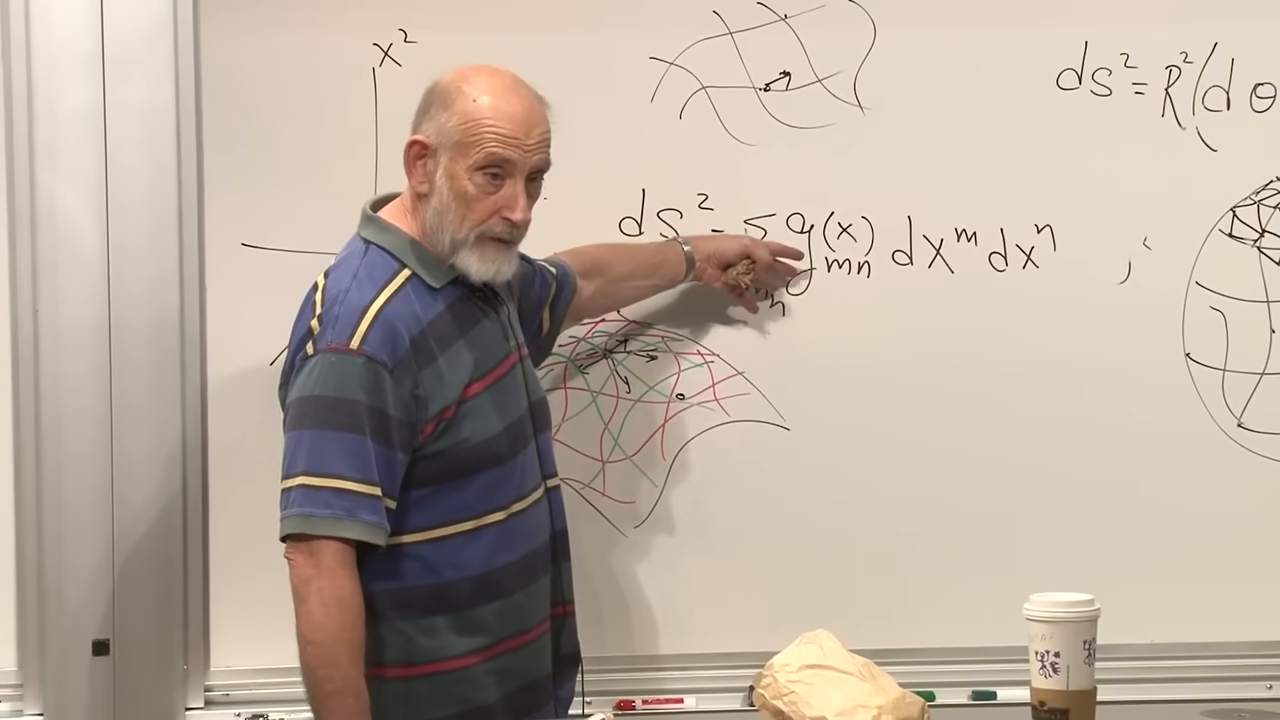
\includegraphics[width=\linewidth]{lecture_01_figure_05.png}
\caption{Các đường cong \(z'\) không đổi đối với hệ tọa độ gia tốc đều.}
\par\smallskip
\textit{Khung hình bài giảng: 00:22:25.}
\end{figure}

Đây là manh mối hình học đầu tiên. Thuyết tương đối hẹp sử dụng các phép biến đổi Lorentz tuyến tính, vốn biến các đường thẳng không-thời gian thành các đường thẳng không-thời gian. Để biểu diễn gia tốc, và do đó bắt chước hấp dẫn, cần các phép biến đổi cong tuyến của tọa độ không-thời gian.

Einstein dùng điểm có vẻ khiêm tốn này để trả lời một câu hỏi hoàn toàn không khiêm tốn: hấp dẫn có ảnh hưởng đến ánh sáng hay không? Tại \(t=0\), cho khung thang máy và khung mặt đất tức thời đứng yên tương đối với nhau, và cho một tia sáng ngang đi qua thang máy. Trong hệ không gia tốc,
\begin{equation}
 x=ct,\qquad z=0.
\end{equation}
Dùng \(z=z'+\tfrac12gt^2\), tia ấy trong tọa độ của thang máy thỏa mãn
\begin{equation}
 z'=-\frac12gt^2
    =-\frac{g}{2c^2}x^2.
\label{eq:accelerated-light}
\end{equation}
Tia sáng là thẳng trong hệ quán tính và cong trong hệ gia tốc. Nếu gia tốc và hấp dẫn tương đương cục bộ, thì một trường hấp dẫn phải bẻ cong ánh sáng. Lập luận này xác lập hiệu ứng đó trước cả khi một phương trình trường cho hấp dẫn được viết ra.

\begin{figure}[H]
\centering
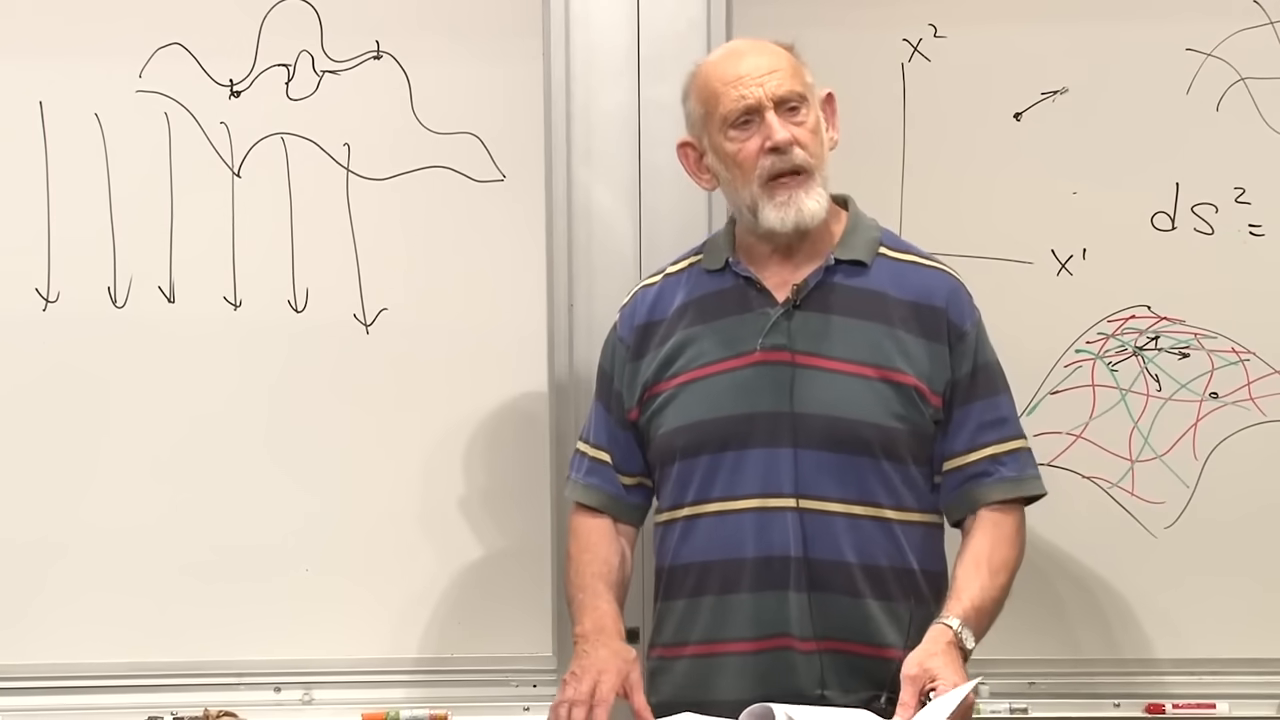
\includegraphics[width=\linewidth]{lecture_01_figure_06.png}
\caption{Tia sáng ngang và quỹ đạo cong của nó trong hệ gia tốc.}
\par\smallskip
\textit{Khung hình bài giảng: 00:28:10.}
\end{figure}

\section{Những gì không thể khử bằng phép biến đổi tọa độ}

Một hệ gia tốc có thể tạo ra một trường hấp dẫn đồng nhất biểu kiến. Từ đó không suy ra rằng mọi trường hấp dẫn đều chỉ là một tạo tác tọa độ. Trường của một ngôi sao hướng vào trong theo phương bán kính. Một phòng thí nghiệm rơi tự do nhỏ gần một điểm có thể xóa gia tốc cục bộ, nhưng cùng phép biến đổi ấy không thể xóa trường ở mọi phía quanh ngôi sao.

\begin{figure}[H]
\centering
\includegraphics[width=\linewidth]{lecture_01_figure_07.png}
\caption{Một trường xuyên tâm và một vật rơi kéo dài dùng để phơi bày gia tốc thủy triều.}
\par\smallskip
\textit{Khung hình bài giảng: 00:32:50.}
\end{figure}

Vật cản trở ở đây là lực thủy triều. Hãy tưởng tượng một người cao hai nghìn dặm rơi với chân xuống trước. Bàn chân của ông ta gần nguồn hơn và gia tốc mạnh hơn đầu, nên ông ta bị kéo dãn ra. Xoay ông ta nằm ngang, và các hướng vào trong ở hai phía đối diện có các thành phần hướng về phía nhau, nên ông ta bị ép lại. Theo ngôn ngữ Newton, các điểm lân cận cách nhau \(\xi^j\) thu được gia tốc tương đối
\begin{equation}
 \delta a^i \simeq \partial_j g^i\,\xi^j.
\label{eq:newtonian-tide}
\end{equation}
Gia tốc tọa độ có thể bị khử. Gia tốc tương đối giữa các phần của một vật rơi tự do có kích thước hữu hạn thì không thể.

\begin{classroomqa}
\audiencequestion{Các động cơ tên lửa khác nhau ở đầu và chân có thể mô phỏng sự kéo dãn ấy và do đó mô phỏng một trường thủy triều không?}
\lecturerresponse{Các động cơ gắn vào dĩ nhiên có thể gây ứng suất lên một vật, nhưng đó là một lực thực, không phải hấp dẫn, tác dụng khác nhau lên các phần của nó. Chỉ riêng một phép đổi tọa độ không thể tạo ra gia tốc tương đối bất biến giữa các hạt rơi tự do lân cận. Dấu hiệu chẩn đoán liên quan đến rơi tự do không bị cưỡng bức, chứ không phải một vật bị đẩy bằng các tên lửa riêng rẽ.
\lecturetimestamp{00:36:51}}
\end{classroomqa}

Tuy vậy, tọa độ cong vẫn có thể làm cho các trường hư cấu trông khá phức tạp. Một hệ có thể gia tốc theo phương thẳng đứng đồng thời dao động theo phương ngang, tạo ra một trường biểu kiến phụ thuộc thời gian với cả hai thành phần. Ngay cả tọa độ cực thông thường cũng cho một ví dụ có tính gợi mở. Một hạt tự do chuyển động trên một đường thẳng Descartes lúc đầu có \(r(t)\) giảm, đạt một bán kính cực tiểu, rồi \(r(t)\) tăng. Ai đó nếu chỉ được cho \(r(t)\) và \(\theta(t)\) có thể suy ra có một lực đẩy ra ngoài. Trong các biến thể quay của những tọa độ này, xuất hiện các hạng ly tâm và Coriolis. Chúng tỉ lệ với khối lượng nên trông giống hấp dẫn, nhưng không để lại biến dạng thủy triều bất biến nào trên một vật rơi tự do.

\begin{classroomqa}
\audiencequestion{Điều gì xảy ra nếu chuyển động được mô tả bằng tọa độ góc hoặc tọa độ cực?}
\lecturerresponse{Mô tả bằng tọa độ phi tuyến làm cho một quỹ đạo tự do thẳng trông như thể bị đẩy ra xa khỏi \(r=0\). Lực ly tâm hiệu dụng ấy là một lực tọa độ. Quay trở lại một hệ tọa độ Descartes quán tính sẽ loại bỏ nó và cho thấy không có biến dạng thủy triều nào.
\lecturetimestamp{00:37:56}}
\end{classroomqa}

\begin{figure}[H]
\centering
\includegraphics[width=\linewidth]{lecture_01_figure_08.png}
\caption{Mô tả bằng tọa độ cực của một quỹ đạo thẳng, với \(r(t)\) và \(\theta(t)\) được ghi trên bảng.}
\par\smallskip
\textit{Khung hình bài giảng: 00:40:20.}
\end{figure}

\begin{classroomqa}
\audiencequestion{Liệu nhiều vật hấp dẫn có thể triệt tiêu lẫn nhau và không để lại lực thủy triều nào không?}
\lecturerresponse{Các lực có thể triệt tiêu tại một điểm được chọn, nhưng việc triệt tiêu giá trị của trường nói chung không triệt tiêu các đạo hàm không gian của nó. Gần bất kỳ nguồn riêng lẻ nào, các quỹ đạo lân cận vẫn có những gia tốc khác nhau. Sự vắng mặt thật sự của độ cong đòi hỏi đại lượng chẩn đoán thủy triều phải triệt tiêu trong toàn bộ vùng, chứ không chỉ lực tổng hợp tại một điểm. \lecturetimestamp{00:42:16}}
\end{classroomqa}

\begin{classroomqa}
\audiencequestion{Về mặt thao tác, lực thủy triều được đo như thế nào?}
\lecturerresponse{Hãy thả rơi tự do một vật có kích thước hữu hạn, chẳng hạn một tinh thể, và quan sát các ứng suất và biến dạng kéo giãn nó theo một phương và nén nó theo phương khác. Những biến dạng đó đo được và không biến mất khi chỉ đổi tên các tọa độ. \lecturetimestamp{00:44:38}}
\end{classroomqa}

\begin{classroomqa}
\audiencequestion{Một người dài hai nghìn dặm trên đu quay có cảm thấy một hiệu ứng thủy triều theo hướng bán kính không?}
\lecturerresponse{Một người bị buộc chặt vào đu quay cảm nhận các lực đỡ và quả thực có thể bị đau đầu. Thay vào đó, vật kiểm tra phải rơi tự do. Quỹ đạo của nó trông phức tạp trong các tọa độ quay nhưng trong hệ quán tính vẫn là một quỹ đạo thẳng không chịu ứng suất, nên lực thủy triều bất biến bằng không.
\lecturetimestamp{00:45:07}}
\end{classroomqa}

\begin{classroomqa}
\audiencequestion{Có thể nghiêng vật đang rơi sao cho sự kéo giãn và sự nén triệt tiêu nhau không?}
\lecturerresponse{Không có một định hướng đơn lẻ nào loại bỏ được toàn bộ biến dạng. Trường hướng tâm kéo giãn theo một phương chính và nén theo các phương ngang. Một vật có kích thước hữu hạn theo mọi phương sẽ chịu toàn bộ mẫu hình đó. \lecturetimestamp{00:47:10}}
\end{classroomqa}

\begin{figure}[H]
\centering
\includegraphics[width=\linewidth]{lecture_01_figure_09.png}
\caption{Sự kéo giãn hướng tâm và sự nén theo phương ngang được minh họa đồng thời cho một vật rơi tự do có kích thước hữu hạn.}
\par\smallskip
\textit{Khung hình bài giảng: 00:47:55.}
\end{figure}

\begin{classroomqa}
\audiencequestion{Các lực thủy triều có nghĩa là nguyên lý tương đương thất bại không?}
\lecturerresponse{Chúng cho thấy nguyên lý ấy phải được phát biểu cẩn thận đến mức nào. Trong một hệ đủ nhỏ để trường hấp dẫn biến thiên không đáng kể trên toàn hệ, hấp dẫn có thể được loại bỏ đến độ chính xác thích hợp bằng một hệ quy chiếu rơi tự do. Phần biến thiên còn dư trên một hệ lớn hơn là trường thủy triều. \lecturetimestamp{00:48:08}}
\end{classroomqa}

\section{Từ hình học Minkowski đến một metric địa phương}

Bây giờ ta tạm rời chủ đề hấp dẫn. Minkowski đã cho thấy rằng không-thời gian có một hình học địa phương bất biến. Trong một chiều không gian, với \(c=1\),
\begin{equation}
 d\tau^2=dt^2-dx^2.
\label{eq:minkowski-proper-time}
\end{equation}
Thay vào đó cũng có thể định nghĩa \(ds^2=dx^2-dt^2=-d\tau^2\). Khác biệt ấy chỉ là quy ước dấu, không phải khác biệt về vật lý.

\begin{classroomqa}
\audiencequestion{Nếu không đặt bằng một, thì tốc độ ánh sáng xuất hiện ở đâu?}
\lecturerresponse{Nếu \(t\) được đo bằng đơn vị thời gian và \(x\) bằng đơn vị độ dài, thì một dạng thuận tiện là
\(d\tau^2=dt^2-dx^2/c^2\). Tương đương, hãy nhân với \(c^2\) và dùng
\(c^2d\tau^2=c^2dt^2-dx^2\). Việc chọn \(ct\) hoặc \(x/c\) làm một tọa độ sẽ hấp thụ hệ số chuyển đổi. \lecturetimestamp{00:51:02}}
\end{classroomqa}

\begin{figure}[H]
\centering
\includegraphics[width=\linewidth]{lecture_01_figure_10.png}
\caption{Khoảng thời gian riêng cung cấp chiếc cầu hình học nối từ thuyết tương đối hẹp đến thuyết tương đối rộng.}
\par\smallskip
\textit{Khung hình bài giảng: 00:51:10.}
\end{figure}

Einstein nhận ra rằng bài toán quyết định liệu một trường hấp dẫn có thể loại bỏ được hay không giống với một bài toán do Gauss nghiên cứu đối với các mặt và do Riemann nghiên cứu trong số chiều tùy ý: cho một quy luật khoảng cách địa phương, làm sao có thể quyết định hình học có thực sự cong hay không?

Trong tọa độ Descartes Euclid, định lý Pythagoras cho
\begin{equation}
 ds^2=(dx^1)^2+(dx^2)^2+\cdots
     =\delta_{mn}\,dx^m dx^n.
\label{eq:euclidean-line-element}
\end{equation}
Miền giá trị của chỉ số là số chiều của không gian. Ký hiệu không thay đổi dù có hai, ba hay hai mươi sáu tọa độ.

\begin{figure}[H]
\centering
\includegraphics[width=\linewidth]{lecture_01_figure_11.png}
\caption{Phần tử đường Euclid dưới dạng tổng các bình phương của các độ tăng tọa độ.}
\par\smallskip
\textit{Khung hình bài giảng: 00:55:00.}
\end{figure}

Đặt các tọa độ tùy ý \(x^m\) trên một mặt tùy ý. Khoảng cách giữa các điểm lân cận là dạng toàn phương
\begin{equation}
 ds^2=g_{mn}(x)\,dx^m dx^n.
\label{eq:general-line-element}
\end{equation}
Các hàm \(g_{mn}(x)\) là các thành phần của tensor metric. Cùng công thức ấy cũng áp dụng cho một bề mặt phẳng được mô tả bằng tọa độ cong; các thành phần metric không hằng tự chúng không chứng minh độ cong nội tại.

\begin{figure}[H]
\centering
\includegraphics[width=\linewidth]{lecture_01_figure_12.png}
\caption{Một dạng toàn phương metric tổng quát bên cạnh một lưới tọa độ cong.}
\par\smallskip
\textit{Khung hình bài giảng: 00:58:20.}
\end{figure}

Đối với một mặt cầu bán kính \(R\), khi \(\theta\) được đo từ một cực,
\begin{equation}
 ds^2=R^2\left(d\theta^2+\sin^2\theta\,d\phi^2\right).
\label{eq:sphere-polar}
\end{equation}
Cùng một độ tăng kinh độ tương ứng với một khoảng cách lớn gần xích đạo và một khoảng cách nhỏ gần một cực; sự phụ thuộc vào vị trí ấy chính là điều mà hệ số ghi lại.

\begin{classroomqa}
\audiencequestion{Vĩ độ thông thường được đo từ xích đạo, vậy hệ số có phải là một cosin thay vì một sin không?}
\lecturerresponse{Đúng. Nếu \(\lambda\) ký hiệu vĩ độ đo từ xích đạo, thì
\(ds^2=R^2(d\lambda^2+\cos^2\lambda\,d\phi^2)\).
Phương trình \eqref{eq:sphere-polar} dùng góc cực
\(\theta=\pi/2-\lambda\), được đo từ cực bắc.
\lecturetimestamp{01:01:03}}
\end{classroomqa}

\begin{figure}[H]
\centering
\includegraphics[width=\linewidth]{lecture_01_figure_13.png}
\caption{Metric của mặt cầu và hình học vĩ độ--kinh độ xác định hệ số phụ thuộc vị trí của nó.}
\par\smallskip
\textit{Khung hình bài giảng: 01:00:30.}
\end{figure}

Các tọa độ tổng quát hơn có thể đưa vào các hạng chéo \(d\theta\,d\phi\),
nhưng khoảng cách địa phương vẫn là bậc hai theo các vi phân. Các hạng bậc ba hoặc bậc một không thuộc về phần tử đường Riemann.

\section{Khoảng cách địa phương và độ cong nội tại}

\begin{classroomqa}
\audiencequestion{Công thức metric có cho luôn khoảng cách giữa hai điểm cách xa nhau không?}
\lecturerresponse{Không, không phải bằng cách thế trực tiếp. Nó cho khoảng cách giữa các điểm lân cận. Một khoảng cách vĩ mô đòi hỏi một đường đi và một tích phân của \(ds\); nếu khoảng cách được hiểu là độ dài của đường đi ngắn nhất, thì bản thân đường đó phải được tìm ra từ hình học. Thậm chí có thể có nhiều đường ngắn nhất cục bộ nối cùng một cặp đầu mút. \lecturetimestamp{01:02:30}}
\end{classroomqa}

Trên một bề mặt gồ ghề, hãy tưởng tượng có các chốt tại hai điểm xa nhau và một sợi dây căng giữa chúng. Sợi dây có thể đi vòng qua phía này hay phía kia của một ngọn đồi, và việc dịch chuyển một ngọn đồi sẽ làm thay đổi lộ trình cực tiểu. Khoảng cách toàn cục phụ thuộc vào hình học ở khoảng giữa. Khoảng cách địa phương đơn giản hơn: metric cung cấp một que nhỏ tại mỗi điểm, và hình học được ghép lại từ những que vô cùng nhỏ ấy.

\begin{figure}[H]
\centering
\includegraphics[width=\linewidth]{lecture_01_figure_14.png}
\caption{Bài toán khoảng cách toàn cục: một đường căng phải tìm đường qua bề mặt giữa hai đầu mút của nó.}
\par\smallskip
\textit{Khung hình bài giảng: 01:04:00.}
\end{figure}

Nếu các mảnh địa phương có thể trải lên một mặt phẳng mà không kéo giãn hay xé rách, thì hình học nội tại là phẳng. Các mảnh có độ dài cạnh của một mặt cầu được tam giác hóa không thể đồng thời trải phẳng mà vẫn giữ nguyên các cạnh của chúng. Vì vậy, metric đặt ra một bài toán chính xác: cho \(g_{mn}(x)\), liệu có thể xác định xem các mảnh vô cùng nhỏ của nó có ghép khít với nhau như một không gian phẳng hay không?

\begin{figure}[H]
\centering
\includegraphics[width=\linewidth]{lecture_01_figure_15.png}
\caption{Metric và mảnh tọa độ địa phương được hiểu như những mảnh vô cùng nhỏ từ đó hình học được lắp ghép.}
\par\smallskip
\textit{Khung hình bài giảng: 01:05:20.}
\end{figure}

\begin{classroomqa}
\audiencequestion{Có thể chẩn đoán độ cong bằng cách đo tỉ số giữa chu vi và đường kính không?}
\lecturerresponse{Có, đó là một phép kiểm tra hai chiều hữu ích. Trên một mặt cong, tỉ số này có thể khác \(\pi\). Tuy nhiên, đối với một đường tròn vô cùng nhỏ, độ lệch chỉ xuất hiện ở bậc cao hơn, và phương pháp này không khái quát gọn gàng bằng tensor độ cong.
\lecturetimestamp{01:07:26}}
\end{classroomqa}

Một miền là phẳng nếu tồn tại một hệ tọa độ trong đó
\begin{equation}
 g_{mn}=\delta_{mn},
\qquad
 ds^2=\delta_{mn}\,dx^m dx^n
\label{eq:flat-metric}
\end{equation}
ở mọi nơi trong miền ấy. Vì thế, một \(g_{mn}(x)\) phức tạp có thể mô tả hoặc một không gian cong, hoặc chỉ đơn thuần là một hệ tọa độ cong trên một không gian phẳng. Câu hỏi là liệu một phép biến đổi tọa độ có thể loại bỏ toàn bộ sự phức tạp đó hay không.

\begin{figure}[H]
\centering
\includegraphics[width=\linewidth]{lecture_01_figure_16.png}
\caption{Bài toán metric được phát biểu trên một mảnh tọa độ địa phương: liệu dạng tọa độ cong của nó có thể được biến đổi thành dạng phẳng hay không?}
\par\smallskip
\textit{Khung hình bài giảng: 01:07:15.}
\end{figure}

\begin{classroomqa}
\audiencequestion{Phần tử độ dài trên mặt cầu có giả định rằng mỗi khoảng rất nhỏ đều có thể xem là phẳng mặc dù bản thân mặt cầu thì không phẳng không?}
\lecturerresponse{Ở bậc dẫn đầu, mọi mặt trơn tại một điểm đều được xấp xỉ bởi mặt phẳng tiếp xúc của nó. Độ cong xuất hiện ở chỗ các xấp xỉ tiếp xúc lân cận không khớp với nhau, hoặc ở những biến thiên bậc cao hơn trên một miền hữu hạn. Vì vậy, tính Euclid cục bộ và độ cong toàn cục là tương thích với nhau. \lecturetimestamp{01:10:01}}
\end{classroomqa}

\begin{classroomqa}
\audiencequestion{Metric có nhất thiết phải liên tục không, và điều gì xảy ra tại một nếp gấp hoặc một khe rãnh?}
\lecturerresponse{Thảo luận này giả sử các ánh xạ tọa độ và một metric đủ trơn để các đạo hàm cần thiết tồn tại. Một tấm được gấp mà không bị kéo giãn có cùng các khoảng cách nội tại ở hai phía của nếp gấp; vẻ ngoài rất ấn tượng của nó là ngoại tại. Một hình học thực sự kỳ dị hoặc không trơn đòi hỏi sự xử lý riêng và nằm ngoài khuôn khổ trơn được dùng ở đây. \lecturetimestamp{01:11:25}}
\end{classroomqa}

Sự phân biệt này chính là hình học nội tại. Uốn cong một trang giấy trong không gian ba chiều làm thay đổi cách nó được nhúng, nhưng không làm thay đổi các khoảng cách đo bên trong trang giấy. Một sinh vật bị giới hạn trên trang giấy, không thể nhìn ra không gian nhúng, vẫn có thể đo hình học nội tại của nó.

\begin{figure}[H]
\centering
\includegraphics[width=\linewidth]{lecture_01_figure_17.png}
\caption{Một tấm giấy gấp được dùng để phân biệt khoảng cách nội tại với biểu hiện ngoại tại.}
\par\smallskip
\textit{Khung hình bài giảng: 01:13:00.}
\end{figure}

\begin{classroomqa}
\audiencequestion{Tại sao không đơn giản chéo hóa metric?}
\lecturerresponse{Tại bất kỳ một điểm nào, một lựa chọn tọa độ thích hợp có thể chéo hóa metric và chuẩn hóa nó về dạng phẳng cục bộ. Trở ngại nằm ở chỗ làm được điều đó trên khắp một miền bằng một hệ tọa độ duy nhất. Không thể phát hiện độ cong chỉ bằng cách xét một điểm đơn lẻ.
\lecturetimestamp{01:13:48}}
\end{classroomqa}

\begin{figure}[H]
\centering
\includegraphics[width=\linewidth]{lecture_01_figure_18.png}
\caption{Metric Descartes phẳng \(\delta_{mn}\) được viết bên dưới dạng toàn phương cục bộ tổng quát.}
\par\smallskip
\textit{Khung hình bài giảng: 01:16:00.}
\end{figure}

Sự tương tự với hấp dẫn giờ đây là chính xác chứ không chỉ mang tính gợi ý. Một lực tọa độ có thể khử được, cũng như một cách mô tả không gian phẳng bằng tọa độ cong có thể khử được. Trong thuyết tương đối rộng, gia tốc thủy triều được đo bằng độ cong. Theo ký hiệu về sau, các đường thế giới rơi tự do lân cận thỏa mãn phương trình độ lệch trắc địa
\begin{equation}
 \frac{D^2\xi^\mu}{D\tau^2}
 =-R^\mu{}_{\nu\rho\sigma}
   u^\nu\xi^\rho u^\sigma.
\label{eq:geodesic-deviation-preview}
\end{equation}
Độ cong bằng không có nghĩa là không có trường thủy triều bất biến; độ cong khác không có nghĩa là không có lựa chọn tọa độ nào có thể khử hấp dẫn trên toàn miền.

\section{Hai hệ tọa độ và một vectơ}

Để quyết định xem một metric có thể được biến đổi thành \(\delta_{mn}\) hay không, trước hết ta phải biết các đối tượng hình học biến đổi như thế nào. Gọi \(x^m\) và \(y^m\) là hai hệ tọa độ trơn trên cùng một miền:
\begin{equation}
 x^m=x^m(y),\qquad y^m=y^m(x).
\label{eq:mutual-coordinate-maps}
\end{equation}
Các ký hiệu \(x\) và \(y\) gắn nhãn cho những hệ tọa độ hoàn chỉnh, chứ không phải hai phương không gian cụ thể.

\begin{figure}[H]
\centering
\includegraphics[width=\linewidth]{lecture_01_figure_19.png}
\caption{Các ánh xạ tọa độ liên hệ lẫn nhau \(x^m(y)\) và
\(y^m(x)\).}
\par\smallskip
\textit{Khung hình bài giảng: 01:20:35.}
\end{figure}

Đối với các điểm lân cận, quy tắc dây chuyền cho
\begin{equation}
 dy^m=\frac{\partial y^m}{\partial x^p}\,dx^p.
\label{eq:differential-transform}
\end{equation}
Chỉ số lặp \(p\) được lấy tổng. Chính độ dời là một vectơ hình học duy nhất; \(dx^p\) và \(dy^m\) là các thành phần của nó trong hai hệ tọa độ.

\begin{figure}[H]
\centering
\includegraphics[width=\linewidth]{lecture_01_figure_20.png}
\caption{Phép biến đổi vi phân của tọa độ thu được từ quy tắc dây chuyền.}
\par\smallskip
\textit{Khung hình bài giảng: 01:22:30.}
\end{figure}

\begin{classroomqa}
\audiencequestion{Trên một lưới tọa độ cong, các đường tọa độ biểu diễn điều gì?}
\lecturerresponse{Trong hai chiều, một đường thu được bằng cách giữ cố định một tọa độ và cho tọa độ kia biến thiên. Trong số chiều cao hơn, các tập hợp tương ứng có tọa độ không đổi là các siêu mặt. Các giao cắt cục bộ của chúng xác định những phương tọa độ dùng để phân giải các thành phần vectơ. \lecturetimestamp{01:25:20}}
\end{classroomqa}

Một vectơ phản biến được định nghĩa bởi cùng quy luật biến đổi như một độ dời tọa độ:
\begin{equation}
 (V')^m(y)
 =\frac{\partial y^m}{\partial x^p}\,V^p(x).
\label{eq:contravariant-vector}
\end{equation}
Vận tốc dọc theo một mặt là một ví dụ. Vectơ không thay đổi khi tọa độ thay đổi; các thành phần của nó thì có.

\begin{figure}[H]
\centering
\includegraphics[width=\linewidth]{lecture_01_figure_21.png}
\caption{Quy luật biến đổi được đóng khung cho một vectơ phản biến.}
\par\smallskip
\textit{Khung hình bài giảng: 01:29:30.}
\end{figure}

Quy ước tổng của Einstein lược bỏ dấu tổng mỗi khi một chỉ số lặp lại một lần ở trên và một lần ở dưới. Quy ước này làm cho các công thức dễ in hơn, nhưng quan trọng hơn, nó làm lộ rõ cấu trúc co.

\begin{classroomqa}
\audiencequestion{Có đang đặt ra giả thiết đặc biệt nào về các hệ tọa độ được phép hay không?}
\lecturerresponse{Chỉ là hai hệ ấy liên hệ với nhau bằng hàm số và đủ trơn để các đạo hàm được viết ra và ánh xạ ngược tồn tại trong miền đang xét. Không giả thiết tính tuyến tính hay tính trực giao. \lecturetimestamp{01:28:12}}
\end{classroomqa}

\section{Đồng vectơ và quy tắc dây chuyền}

Gọi \(S(x)\) là một vô hướng: nó có một giá trị xác định duy nhất tại mỗi điểm, không phụ thuộc vào các nhãn tọa độ. Nhiệt độ và một trường vô hướng là các ví dụ. Gradient của nó có các thành phần
\begin{equation}
 W_p=\frac{\partial S}{\partial x^p}.
\label{eq:gradient-covector}
\end{equation}

\begin{figure}[H]
\centering
\includegraphics[width=\linewidth]{lecture_01_figure_22.png}
\caption{Gradient của một vô hướng được đưa vào bên cạnh quy luật biến đổi của vectơ phản biến.}
\par\smallskip
\textit{Khung hình bài giảng: 01:31:40.}
\end{figure}

Áp dụng quy tắc dây chuyền trong hệ tọa độ \(y\),
\begin{equation}
 W'_m
 =\frac{\partial S}{\partial y^m}
 =\frac{\partial x^p}{\partial y^m}
  \frac{\partial S}{\partial x^p}
 =\frac{\partial x^p}{\partial y^m}\,W_p.
\label{eq:covariant-vector}
\end{equation}
Đây là quy luật biến đổi của một vectơ hiệp biến, hay đồng vectơ. Jacobian là nghịch đảo của cái trong
\eqref{eq:contravariant-vector}; vì vậy, chỉ số dưới và chỉ số trên mã hóa những cách biến đổi khác nhau.

\begin{figure}[H]
\centering
\includegraphics[width=\linewidth]{lecture_01_figure_23.png}
\caption{Các quy luật biến đổi phản biến và hiệp biến được trình bày cùng nhau.}
\par\smallskip
\textit{Khung hình bài giảng: 01:34:40.}
\end{figure}

\begin{classroomqa}
\audiencequestion{Mối liên hệ giữa vectơ hiệp biến và vectơ phản biến là gì?}
\lecturerresponse{Ở giai đoạn này, chúng được định nghĩa là những loại đối tượng khác nhau: các độ dời và vận tốc biến đổi theo một cách, còn gradient thì theo cách ngược lại. Metric về sau sẽ cung cấp một ánh xạ một-một để hạ hoặc nâng một chỉ số. Không nên giả định mối liên hệ đó trước khi metric được đưa vào. \lecturetimestamp{01:37:43}}
\end{classroomqa}

\begin{classroomqa}
\audiencequestion{Trước đây, việc hạ một chỉ số có làm đổi dấu thành phần thời gian không?}
\lecturerresponse{Dấu đó xuất phát từ metric Lorentz. Phép suy ra hiện tại trước hết được thực hiện trong hình học Euclid thông thường. Việc nâng hay hạ chỉ số luôn dùng metric thích hợp; dấu của thành phần thời gian chỉ xuất hiện khi metric đó có chữ ký Lorentz.
\lecturetimestamp{01:38:29}}
\end{classroomqa}

\begin{classroomqa}
\audiencequestion{Liệu hai quy luật biến đổi ấy đã nên được xem là hai cách mô tả thành phần của cùng một vectơ chưa?}
\lecturerresponse{Chưa. Khi đã có metric, một vectơ phản biến \(V^m\) có thể được chuyển thành một đồng vectơ
\(V_m=g_{mn}V^n\). Cho đến khi ánh xạ đó được thiết lập, các đối tượng mang chỉ số trên và chỉ số dưới là khác biệt về mặt logic. \lecturetimestamp{01:39:00}}
\end{classroomqa}

Các công thức này không phụ thuộc vào số chiều. Miền giá trị của chỉ số thay đổi, nhưng các quy luật biến đổi thì không.

\section{Tensor với hơn một chỉ số}

Xét hai vectơ phản biến \(V^m\) và \(U^n\). Tích của chúng
\begin{equation}
 T^{mn}=V^mU^n
\label{eq:rank-two-product}
\end{equation}
là một tensor phản biến hạng hai. Trong ba chiều nó có chín thành phần; trong bốn chiều nó có mười sáu thành phần. Thứ tự của các chỉ số là quan trọng, trừ khi có cho trước một đối xứng riêng: \(T^{mn}\) không nhất thiết bằng
\(T^{nm}\).

\begin{figure}[H]
\centering
\includegraphics[width=\linewidth]{lecture_01_figure_24.png}
\caption{Một tensor hạng hai được tạo thành như tích của hai vectơ phản biến.}
\par\smallskip
\textit{Khung hình bài giảng: 01:43:40.}
\end{figure}

Mỗi chỉ số trên đóng góp một Jacobian thuận:
\begin{equation}
 (T')^{mn}
 =\frac{\partial y^m}{\partial x^p}
  \frac{\partial y^n}{\partial x^q}
  T^{pq}.
\label{eq:rank-two-contravariant}
\end{equation}
Cách xây dựng bằng tích gợi ra quy tắc này, nhưng quy luật biến đổi mới là định nghĩa của một tensor. Một tensor phản biến hạng ba sẽ có ba thừa số Jacobian như vậy.

\begin{figure}[H]
\centering
\includegraphics[width=\linewidth]{lecture_01_figure_25.png}
\caption{Hai thừa số Jacobian trong phép biến đổi của
\(T^{mn}\).}
\par\smallskip
\textit{Khung hình bài giảng: 01:44:20.}
\end{figure}

Tương tự, mỗi chỉ số dưới đóng góp một Jacobian nghịch đảo:
\begin{equation}
 T'_{mn}
 =\frac{\partial x^p}{\partial y^m}
  \frac{\partial x^q}{\partial y^n}
  T_{pq}.
\label{eq:rank-two-covariant}
\end{equation}
Một tensor hỗn hợp dùng một thừa số của mỗi loại.

\begin{figure}[H]
\centering
\includegraphics[width=\linewidth]{lecture_01_figure_26.png}
\caption{Quy luật biến đổi đầy đủ cho một tensor với hai chỉ số hiệp biến.}
\par\smallskip
\textit{Khung hình bài giảng: 01:47:30.}
\end{figure}

Bây giờ cùng một bộ máy biến đổi được áp dụng cho metric. Vì phần tử độ dài là một vô hướng, nó phải có cùng một giá trị trong cả hai hệ tọa độ:
\begin{align}
 ds^2
 &=g_{mn}(x)\,dx^m dx^n,\\
 dx^m
 &=\frac{\partial x^m}{\partial y^p}\,dy^p.
\end{align}
Phép thế hoàn tất dòng mà bảng còn để dở:
\begin{equation}
 g'_{pq}(y)
 =\frac{\partial x^m}{\partial y^p}
  \frac{\partial x^n}{\partial y^q}
  g_{mn}(x(y)).
\label{eq:l1-metric-transformation}
\end{equation}
Vì thế \(g_{mn}\) là một tensor hiệp biến hạng hai.

\begin{figure}[H]
\centering
\includegraphics[width=\linewidth]{lecture_01_figure_27.png}
\caption{Phép biến đổi của metric được khởi đầu từ tính bất biến của phần tử độ dài ở cuối bài giảng.}
\par\smallskip
\textit{Khung hình bài giảng: 01:48:40.}
\end{figure}

Câu hỏi vật lý mở đầu nay đã trở thành một câu hỏi toán học. Cho \(g_{mn}(x)\), có tồn tại một phép biến đổi tọa độ sao cho \(g'_{mn}=\delta_{mn}\) trên toàn miền hay không? Nếu có, sự phức tạp biểu kiến chỉ là sự phức tạp của tọa độ. Nếu không, vật cản đó là độ cong, và trong không-thời gian, chính vật cản ấy là nội dung bất biến của hấp dẫn.
